\documentclass[10pt, aspectratio=169]{beamer}
\usetheme{Madrid}

% ============================================================================
% OPCIÓN DE COLOR: Cambia el valor de la siguiente línea para modificar el color
% ============================================================================
% Verde cálido/oscuro actual: #2E7D32 (un verde bosque)
% Alternativas sugeridas:
%   Verde oliva:   #556B2F
%   Verde militar: #4A5D23  
%   Verde musgo:   #5C6E38
%   Verde pino:    #2C5F2D
%   Verde jade:    #2F6B47
\definecolor{miVerde}{RGB}{46,125,50}  % #2E7D32 - Verde bosque
\definecolor{blanco}{RGB}{244,202,244}  % #90C990 - Verde claro para acentos
% ============================================================================

% Configurar el color en el tema Madrid
\setbeamercolor{title}{fg=blanco}
\setbeamercolor{frametitle}{fg=blanco}
\setbeamercolor{structure}{fg=miVerde}
\setbeamercolor{block title}{bg=miVerde!80!black, fg=white}
\setbeamercolor{block body}{bg=miVerde!10}
\setbeamercolor{alerted text}{fg=miVerde!70!black}
\setbeamercolor{section in toc}{fg=miVerde!80!black}

% Cambiar el color de los bullets y números
\setbeamercolor{item}{fg=miVerde}
\setbeamercolor{subitem}{fg=miVerde!70}

% Cambiar el color de la barra superior (headline) del tema Madrid
\setbeamercolor{headline}{fg=white, bg=miVerde!60!black}

% Paquetes necesarios
\usepackage[utf8]{inputenc}
\usepackage{amsmath, amssymb, amsfonts}
\usepackage{graphicx}
\usepackage{tikz}
\usetikzlibrary{positioning, arrows.meta}
\usepackage{booktabs}
\usepackage{hyperref}

% ÍNDICE GENERAL: Solo aparece UNA VEZ al inicio (sin secciones automáticas)
% Para que no genere diapositivas por cada cambio de tema, eliminamos el \AtBeginSection

% Título y autor
\title[AGs en Espacios Métricos]{Algoritmos Genéticos en Espacios Métricos\\ {\small De $\mathbb{R}^n$ a la Convergencia Débil}}
\author{C. Fabián Beltrán I.}
\institute{Matemáticas Aplicadas y Computación}
\date{03 de Junio}

\begin{document}

% ============================================================================
% Portada
% ============================================================================
\begin{frame}
\titlepage
\centering
\textbf{BLX-$\alpha$ y Mutación Gaussiana}
\end{frame}

% ============================================================================
% ÍNDICE GENERAL (ÚNICA VEZ, SIN SUBDIVISIONES AUTOMÁTICAS)
% ============================================================================
\begin{frame}{Índice general}
\tableofcontents
\end{frame}

% ============================================================================
% SECCIÓN 1: INTRODUCCIÓN Y MOTIVACIÓN
% ============================================================================
\section{Introducción y Motivación}

% Diapositiva 1.1: Motivación
\begin{frame}{Motivación}
\begin{itemize}
    \item \textbf{Problemas reales} tienen variables \alert{continuas}
    \begin{itemize}
        \item Pesos, coordenadas, parámetros físicos
        \item Funciones, curvas, superficies
    \end{itemize}
    \item \textbf{Codificación binaria}:
    \begin{itemize}
        \item Requiere discretización $\rightarrow$ pérdida de precisión
        \item Espacio de búsqueda finito pero enorme
    \end{itemize}
    \item \textbf{Ventaja de la codificación real}:
    \begin{itemize}
        \item Respeta la topología del espacio
        \item Operadores naturales (mutación gaussiana)
    \end{itemize}
\end{itemize}
\rule{\textwidth}{0.5pt}
\vspace{2mm}
\footnotesize \textcolor{gray}{Nota: La codificación real trabaja directamente con el valor de $\theta$ (el genotipo), sin una "codificación" en el sentido binario.}
\end{frame}

% Diapositiva 1.2: Espacio de búsqueda y métrica
\begin{frame}{Espacio de búsqueda y su estructura}
\begin{block}{Espacio de genotipos}
\[
\mathcal{X} \subseteq \mathbb{R}^n \quad \text{(subconjunto acotado o todo $\mathbb{R}^n$)}
\]
\end{block}

\begin{block}{Espacio de poblaciones (con $N$ individuos)}
\[
\mathcal{X}^N = \underbrace{\mathcal{X} \times \mathcal{X} \times \cdots \times \mathcal{X}}_{N \text{ veces}}
\]
\end{block}

\begin{block}{Distancia (métrica) para definir vecindad y convergencia}
\[
d(\mathbf{x}, \mathbf{y}) = \|\mathbf{x} - \mathbf{y}\|_2 = \sqrt{\sum_{i=1}^n (x_i - y_i)^2}
\]
\end{block}
\end{frame}

% Diapositiva 1.3: Definición formal de espacio métrico
\begin{frame}{Definición: Espacio Métrico}
Un espacio métrico es una pareja $(X, d)$ donde $X$ es un conjunto y $d$ es una función de distancia que satisface:

\begin{enumerate}
    \item \textbf{No negatividad y definida positiva:} 
    \[
    d(x,y) \ge 0 \quad \text{y} \quad d(x,y)=0 \iff x=y
    \]
    \item \textbf{Simetría:} 
    \[
    d(x,y) = d(y,x)
    \]
    \item \textbf{Desigualdad triangular:} 
    \[
    d(x,z) \le d(x,y) + d(y,z)
    \]
\end{enumerate}

\vspace{2mm}
\rule{\textwidth}{0.5pt}
\vspace{2mm}
\footnotesize \textcolor{gray}{Nota: Todo espacio normado es métrico (con $d(x,y)=\|x-y\|$), pero no todo espacio métrico es normado.}
\end{frame}

% ============================================================================
% SECCIÓN 2: OPERADORES EN CÓDIFICACIÓN REAL
% ============================================================================
\section{Operadores en Codificación Real}

% Diapositiva 2.1: Cruce BLX-α
\begin{frame}{Operadores: Cruce BLX-$\alpha$}
\begin{block}{Definición}
Dados dos padres $\mathbf{p}, \mathbf{q} \in \mathbb{R}^n$, para cada coordenada $i$ se define:
\[
d_i = |p_i - q_i|
\]
\[
\text{intervalo} = [\min(p_i, q_i) - \alpha d_i,\; \max(p_i, q_i) + \alpha d_i]
\]
% El hijo se genera tomando cada coordenada $h_i$ \textbf{uniformemente} en ese intervalo.
\end{block}

\begin{block}{Interpretación gráfica}
\centering
% \begin{tikzpicture}[scale=0.8]
%     \draw[thick, blue] (0,0) -- (6,0);
%     \draw[thick, red] (1,0.1) -- (5,-0.1);
%     \draw[->, thick] (0.5,0.5) -- (1.5,0.5) node[midway, above] {$\alpha=0$};
%     \draw[->, thick] (3.5,0.5) -- (5.5,0.5) node[midway, above] {$\alpha=0.5$};
% \end{tikzpicture}
\includegraphics[width=0.4\textwidth]{imgs/blx.png}
\end{block}

\begin{itemize}
    \item $\alpha \ge 0$ (típicamente $\alpha = 0.5$)
    \item Controla la exploración fuera del intervalo de los padres
\end{itemize}
\end{frame}

% Diapositiva 2.2: Mutación Gaussiana
\begin{frame}{Operadores: Mutación Gaussiana}
\begin{block}{Definición}
Dado un individuo $\mathbf{y} \in \mathbb{R}^n$, el individuo mutado es:
\[
\tilde{\mathbf{y}} = \mathbf{y} + \mathbf{z}
\]
donde $\mathbf{z} = \sigma \big( \mathcal{N}_1(0,1), \dots, \mathcal{N}_n(0,1) \big)$.
\end{block}

\begin{itemize}
    \item $\sigma$: intensidad de mutación (parámetro de escala)
    \item $\mathcal{N}_i(0,1)$: normales estándar independientes
    \item \textbf{Soporte completo} en $\mathbb{R}^n$ (puede alcanzar cualquier punto)
\end{itemize}

\vspace{2mm}
\rule{\textwidth}{0.5pt}
\vspace{2mm}
\footnotesize \textcolor{gray}{Nota: Por el principio de máxima entropía, para media y varianza fijas, la distribución normal es la que maximiza la entropía, lo que la hace ideal para una exploración no sesgada.}
\end{frame}

% ============================================================================
% SECCIÓN 3: MODELADO ESTOCÁSTICO
% ============================================================================
\section{Modelado Estocástico}

% Diapositiva 3.1: Medida empírica
\begin{frame}{Modelado de la población: Medida empírica}
\begin{block}{Población en tiempo $t$}
\[
P_t = \{\mathbf{x}_1^{(t)}, \mathbf{x}_2^{(t)}, \dots, \mathbf{x}_N^{(t)}\} \subset \mathbb{R}^n
\]
\end{block}

\begin{block}{Medida empírica asociada}
\[
\mu_t^N = \frac{1}{N} \sum_{i=1}^N \delta_{\mathbf{x}_i^{(t)}}
\]
donde $\delta_{\mathbf{x}}$ es la masa de Dirac en $\mathbf{x}$.
\end{block}

\begin{itemize}
    \item $\mu_t^N$ es una \alert{medida de probabilidad} sobre $\mathbb{R}^n$
    \item Describe la \textbf{distribución} de la población en el espacio
    \item $\mu_t^N(A)$ = proporción de individuos en $A \subseteq \mathbb{R}^n$
    \item Permite \textbf{comparar poblaciones} de diferente tamaño
\end{itemize}
\end{frame}

% Diapositiva 3.2: Kernel de Markov
\begin{frame}{Evolución como Kernel de Markov}
\begin{block}{Kernel de transición}
El AG define un kernel $K_N$ que actúa sobre medidas empíricas:
\[
\mu_{t+1}^N = K_N(\mu_t^N)
\]
\end{block}

\begin{block}{Componentes del kernel $K_N$}
\begin{itemize}
    \item \textbf{Selección:} proporcional al fitness (ruleta, torneo)
    \item \textbf{Cruce:} BLX-$\alpha$ (extiende el intervalo entre padres)
    \item \textbf{Mutación:} Gaussiana $\mathbf{x}' = \mathbf{x} + \mathcal{N}(\mathbf{0}, \sigma^2 I)$
\end{itemize}
\end{block}

\vspace{2mm}
\centering
\alert{$P_t \xrightarrow{\text{Selección}} \xrightarrow{\text{Cruce}} \xrightarrow{\text{Mutación}} P_{t+1}$}
\end{frame}

% ============================================================================
% SECCIÓN 4: LÍMITE DE CAMPO MEDIO
% ============================================================================
\section{Límite de Campo Medio}

% Diapositiva 4.1: Definición y teorema
\begin{frame}{Límite de campo medio ($N \to \infty$)}
\begin{block}{Comportamiento asintótico}
Cuando el tamaño de población $N$ tiende a infinito, la medida empírica $\mu_t^N$ \textbf{converge} (en probabilidad) a una medida determinista $\mu_t$ que satisface:
\[
\mu_{t+1} = K(\mu_t)
\]
\end{block}

\begin{theorem}[Champagnat, Ferrière \& Méléard, 2006]
En el límite $N \to \infty$, la evolución de la población sigue la ecuación:
\[
\frac{\partial}{\partial t} \mu_t = \underbrace{\text{Selección}[\mu_t]}_{\text{replicador}} + \underbrace{\text{Cruce}[\mu_t]}_{\text{mezcla}} + \underbrace{\text{Mutación}[\mu_t]}_{\text{difusión}}
\]
\end{theorem}
\end{frame}

% Diapositiva 4.2: Interpretación
\begin{frame}{¿Qué significa el límite de campo medio?}
\begin{itemize}
    \item El \textbf{ruido} estocástico desaparece en el límite
    \item La dinámica se vuelve \alert{determinista}
    \item Se obtiene una \textbf{ecuación de evolución} (no lineal, por la selección)
\end{itemize}

\vspace{3mm}
\centering
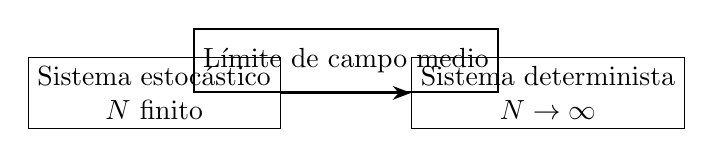
\begin{tikzpicture}[node distance=1cm, auto, 
    every node/.style={rectangle, draw, minimum width=3cm, minimum height=0.8cm, align=center}]
    \node (estocastico) {Sistema estocástico\\$N$ finito};
    \node (determinista) [right of=estocastico, xshift=4cm] {Sistema determinista\\$N \to \infty$};
    \draw[->, thick, -{Stealth}] (estocastico) -- node[above] {Límite de campo medio} (determinista);
\end{tikzpicture}

\vspace{3mm}
\rule{\textwidth}{0.5pt}
\vspace{2mm}
\footnotesize \textcolor{gray}{Analogía física: Un gas con muchas moléculas tiene un comportamiento promedio (presión, temperatura) determinista, aunque las moléculas individuales se muevan aleatoriamente.}
\end{frame}

% ============================================================================
% SECCIÓN 5: CONVERGENCIA DÉBIL
% ============================================================================
\section{Convergencia Débil}

% Diapositiva 5.1: Condiciones y teorema
\begin{frame}{Convergencia débil de $\mu_t$}
\begin{block}{Condiciones suficientes}
\begin{itemize}
    \item Fitness \textbf{continuo} y acotado
    \item Mutación \textbf{gaussiana} $\Rightarrow$ \alert{soporte completo} en $\mathbb{R}^n$
    \item $\alpha \ge 0$ en BLX-$\alpha$ (típicamente $\alpha = 0.5$)
    \item Elitismo (opcional, acelera la convergencia)
\end{itemize}
\end{block}

\begin{theorem}[Convergencia débil]
Bajo estas condiciones, $\mu_t$ converge débilmente a una distribución límite $\mu_\infty$:
\[
\int f(\mathbf{x})\, d\mu_t(\mathbf{x}) \xrightarrow{t \to \infty} \int f(\mathbf{x})\, d\mu_\infty(\mathbf{x})
\]
para toda función $f$ continua y acotada.
\end{theorem}
\end{frame}

% Diapositiva 5.2: Interpretación y relación con Cerf
\begin{frame}{Interpretación y el Teorema de Cerf}
\begin{block}{¿Qué significa convergencia débil?}
La población no colapsa necesariamente a un solo punto, sino que su \textbf{distribución} tiende a una distribución límite.
\end{block}

\begin{block}{Ejemplo}
Si $f$ vale 1 cerca del óptimo y 0 lejos:
\[
\int f(\mathbf{x})\, d\mu_t(\mathbf{x}) = \text{proporción de individuos cerca del óptimo} \to 1
\]
\end{block}

\begin{theorem}[Cerf, 1998]
Bajo condiciones similares (mutación positiva, espacio compacto, fitness continuo):
\[
\mathbb{P}\left( \lim_{t \to \infty} \|\mathbf{x}_{\text{mejor}}^{(t)} - \mathbf{x}^*\| = 0 \right) = 1
\]
\alert{Convergencia casi segura} (más fuerte que la débil).
\end{theorem}
\end{frame}

% Diapositiva 5.3: Distribuciones continuas como límite
\begin{frame}{Distribuciones continuas como límite}
\begin{block}{¿Por qué "distribuciones continuas"?}
\begin{itemize}
    \item El espacio de búsqueda $\mathbb{R}^n$ es continuo
    \item La mutación gaussiana produce \textbf{densidades continuas}
    \item $\mu_\infty$ suele ser una \alert{distribución de Gibbs}:
    \[
    \mu_\infty(d\mathbf{x}) \propto e^{F(\mathbf{x})/\tau} \, d\mathbf{x}
    \]
\end{itemize}
\end{block}

\begin{block}{Concentración en el óptimo}
\begin{itemize}
    \item Fitness con único máximo global $\Rightarrow$ $\mu_\infty = \delta_{\mathbf{x}^*}$ (masa de Dirac)
    \item Múltiples óptimos $\Rightarrow$ $\mu_\infty$ es una \textbf{mezcla} de masas
\end{itemize}
\end{block}
\end{frame}

% ============================================================================
% SECCIÓN 6: ESQUEMA Y LIMITACIONES
% ============================================================================
\section{Esquema y Limitaciones}

% Diapositiva 6.1: Esquema visual
\begin{frame}{Esquema del desarrollo}
\centering
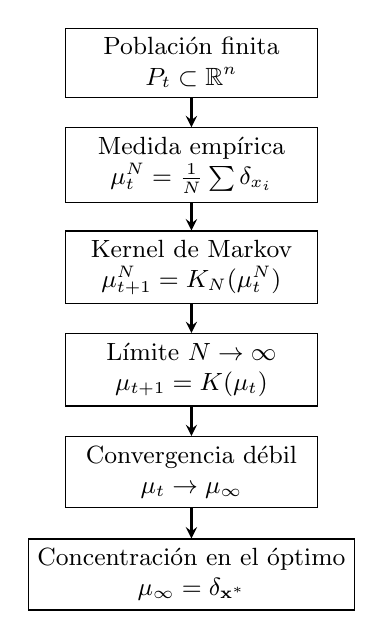
\begin{tikzpicture}[node distance=1.3cm, auto, 
    every node/.style={rectangle, draw, minimum width=3.2cm, minimum height=0.8cm, align=center, font=\small}]
    
    \node (poblacion) {Población finita\\$P_t \subset \mathbb{R}^n$};
    \node (medida) [below of=poblacion] {Medida empírica\\$\mu_t^N = \frac{1}{N}\sum \delta_{x_i}$};
    \node (kernel) [below of=medida] {Kernel de Markov\\$\mu_{t+1}^N = K_N(\mu_t^N)$};
    \node (campo) [below of=kernel] {Límite $N \to \infty$\\$\mu_{t+1} = K(\mu_t)$};
    \node (debil) [below of=campo] {Convergencia débil\\$\mu_t \to \mu_\infty$};
    \node (optimo) [below of=debil] {Concentración en el óptimo\\$\mu_\infty = \delta_{\mathbf{x}^*}$};

    \draw[->, >=stealth, thick] (poblacion) -- (medida);
    \draw[->, >=stealth, thick] (medida) -- (kernel);
    \draw[->, >=stealth, thick] (kernel) -- (campo);
    \draw[->, >=stealth, thick] (campo) -- (debil);
    \draw[->, >=stealth, thick] (debil) -- (optimo);
    
\end{tikzpicture}

\vspace{3mm}
\centering
\alert{Objetivo:} Mostrar que la población se aproxima al óptimo en distribución
\end{frame}

% Diapositiva 6.2: Limitaciones y desafíos
\begin{frame}{Limitaciones y desafíos abiertos}
\begin{itemize}
    \item \alert{Maldición de la dimensionalidad}
    \begin{itemize}
        \item El volumen del espacio crece exponencialmente con $n$
        \item Se necesitan poblaciones muy grandes
    \end{itemize}
    \item \alert{Selección del paso de mutación $\sigma$}
    \begin{itemize}
        \item Trade-off entre exploración y explotación
        \item Estrategias adaptativas (autoadaptación)
    \end{itemize}
    \item \alert{Convergencia a óptimos locales}
    \begin{itemize}
        \item Problemas multimodales
        \item Técnicas de niching
    \end{itemize}
    \item \alert{Análisis teórico} más complejo que en caso binario
    \begin{itemize}
        \item Espacio de estados no numerable
        \item Operadores continuos vs. discretos
    \end{itemize}
\end{itemize}
\end{frame}

% ============================================================================
% SECCIÓN 7: COMPARACIÓN Y CONCLUSIÓN
% ============================================================================
\section{Comparación y Conclusión}

% Diapositiva 7.1: Tabla comparativa
\begin{frame}{Comparación con otros métodos}
\begin{table}
\centering
\begin{tabular}{lccc}
\toprule
\textbf{Método} & \textbf{Espacio} & \textbf{Ventajas} & \textbf{Desventajas} \\
\midrule
AG binario & $\{0,1\}^n$ & Teoría madura & Mala precisión en continuo \\
AG real & $\mathbb{R}^n$ & Natural para continuo & Análisis complejo \\
Recocido simulado & $\mathbb{R}^n$ & Convergencia garantizada & Lento, sin población \\
Enjambre de partículas & $\mathbb{R}^n$ & Paralelizable & Menos teoría de convergencia \\
Estrategias evolutivas & $\mathbb{R}^n$ & Adaptación de parámetros & Complejidad de implementación \\
\bottomrule
\end{tabular}
\end{table}
\vspace{2mm}
\footnotesize \textcolor{gray}{Nota: Los AGs reales son especialmente útiles cuando la función objetivo es continua pero no diferenciable, o cuando el espacio de búsqueda es de alta dimensión.}
\end{frame}

% Diapositiva 7.2: Conclusión
\begin{frame}{Conclusiones y referencias}
\begin{block}{Conclusiones}
\begin{enumerate}
    \item Los AGs en espacios métricos generales son herramientas poderosas para \alert{optimización continua}
    \item Su análisis requiere \alert{cadenas de Markov en espacios continuos} y \alert{teoría de medidas}
    \item El límite de campo medio y la convergencia débil proporcionan un marco riguroso
    \item Quedan desafíos abiertos: alta dimensionalidad, adaptación de parámetros
\end{enumerate}
\end{block}

\begin{block}{Referencias clave}
\begin{itemize}
    \item Beyer, H.G. \& Schwefel, H.P. (2002). \textit{Evolution strategies – A comprehensive introduc-
tion. Natural Computing}
    \item Spall, J.C. (2003). \textit{Introduction to stochastic search and optimization. Wiley}
    \item Chang, F. J. \& Chen, L. (1998). \textit{Real-Coded Genetic Algorithm for Rule-Based.
Flood Control Reservoir Management}
    % \item Champagnat, N. et al. (2006). \textit{Theoretical Population Biology}
\end{itemize}
\end{block}
\end{frame}

% ============================================================================
% SECCIÓN 8: CIERRE
% ============================================================================
\section{Cierre}

% Diapositiva final
\begin{frame}{}

\huge Gracias por su atención
\end{frame}

\end{document}